\documentclass[a4paper,12pt]{article}
%\documentclass[a4paper,12pt]{scrartcl}

% Useful packages for physics experiments
\usepackage[utf8]{inputenc}   % file encoding
\usepackage[T1]{fontenc}      % proper font encoding
\usepackage[english]{babel}   % document language
\usepackage{amsmath, amssymb} % mathematics
\usepackage{graphicx}         % images
\usepackage{siunitx}          % units
\usepackage{hyperref}         % PDF links
\usepackage{csvsimple}
\usepackage{booktabs}
\usepackage{fontspec}   % dla XeLaTeX lub LuaLaTeX
\setmainfont{Times New Roman} % lub inna czcionka obsługująca Δ
\usepackage{float}
\usepackage{tabularx}
\usepackage[a4paper, margin=2.5cm]{geometry}
\usepackage{sectsty}
\usepackage{microtype}
%\usepackage{lmodern}  % Latin Modern, ładna nowoczesna czcionka
\allsectionsfont{\sffamily\bfseries} % wszystkie nagłówki pogrubione i bezszeryfowe
\usepackage{titling}
\pretitle{\begin{center}\Huge\bfseries}
\posttitle{\end{center}}

\setlength{\tabcolsep}{12pt} % odstęp między kolumnami
\renewcommand{\arraystretch}{1.2} % wysokość wierszy

\title{Linear Thermal Expansion Experiment}
\author{Roland Sobczak}
\date{\today}

\begin{document}

\maketitle

\section{Introduction}

The aim of this experiment is to investigate the phenomenon of linear thermal expansion of solid materials and to determine the linear expansion coefficient of the tested materials.

Thermal expansion is the change in the dimensions of a body due to a change in temperature. For small temperature changes, the length of a body changes proportionally to the temperature difference, according to the relation:
\begin{equation}
    \Delta L = \alpha \, L_0 \, \Delta T
\end{equation}
where:
\begin{itemize}
    \item $\Delta L$ – change in length,
    \item $L_0$ – initial length of the body,
    \item $\Delta T$ – temperature change,
    \item $\alpha$ – linear expansion coefficient.
\end{itemize}

This experiment allows us to verify this relationship and determine the value of $\alpha$ for metals, which is important when designing structures exposed to temperature variations.

\section{Experimental Procedure}

During the experiment, the lengths of rods made from three different metals were measured:
\begin{enumerate}
    \item Copper
    \item Brass
    \item Steel
\end{enumerate}

The procedure was as follows:

\begin{enumerate}
    \item First, the initial absolute length of each rod was measured. The measuring device had an accuracy of 0.05 mm. The initial temperature was 24.2°C.
    \item Next, the temperature was increased in steps of 5°C and the change in length relative to the initial length was measured. Measurements were done with an accuracy of 0.01 mm.
    \item For simplification, measurements were performed at slightly different temperatures for each rod. The exact temperature for each measurement is reported in the results. The thermometer had an accuracy of 0.1°C.
\end{enumerate}

\section{Results}

The following section presents the measured data and the calculated linear expansion coefficients for the three metals.

\begin{figure}[h]
    \centering
    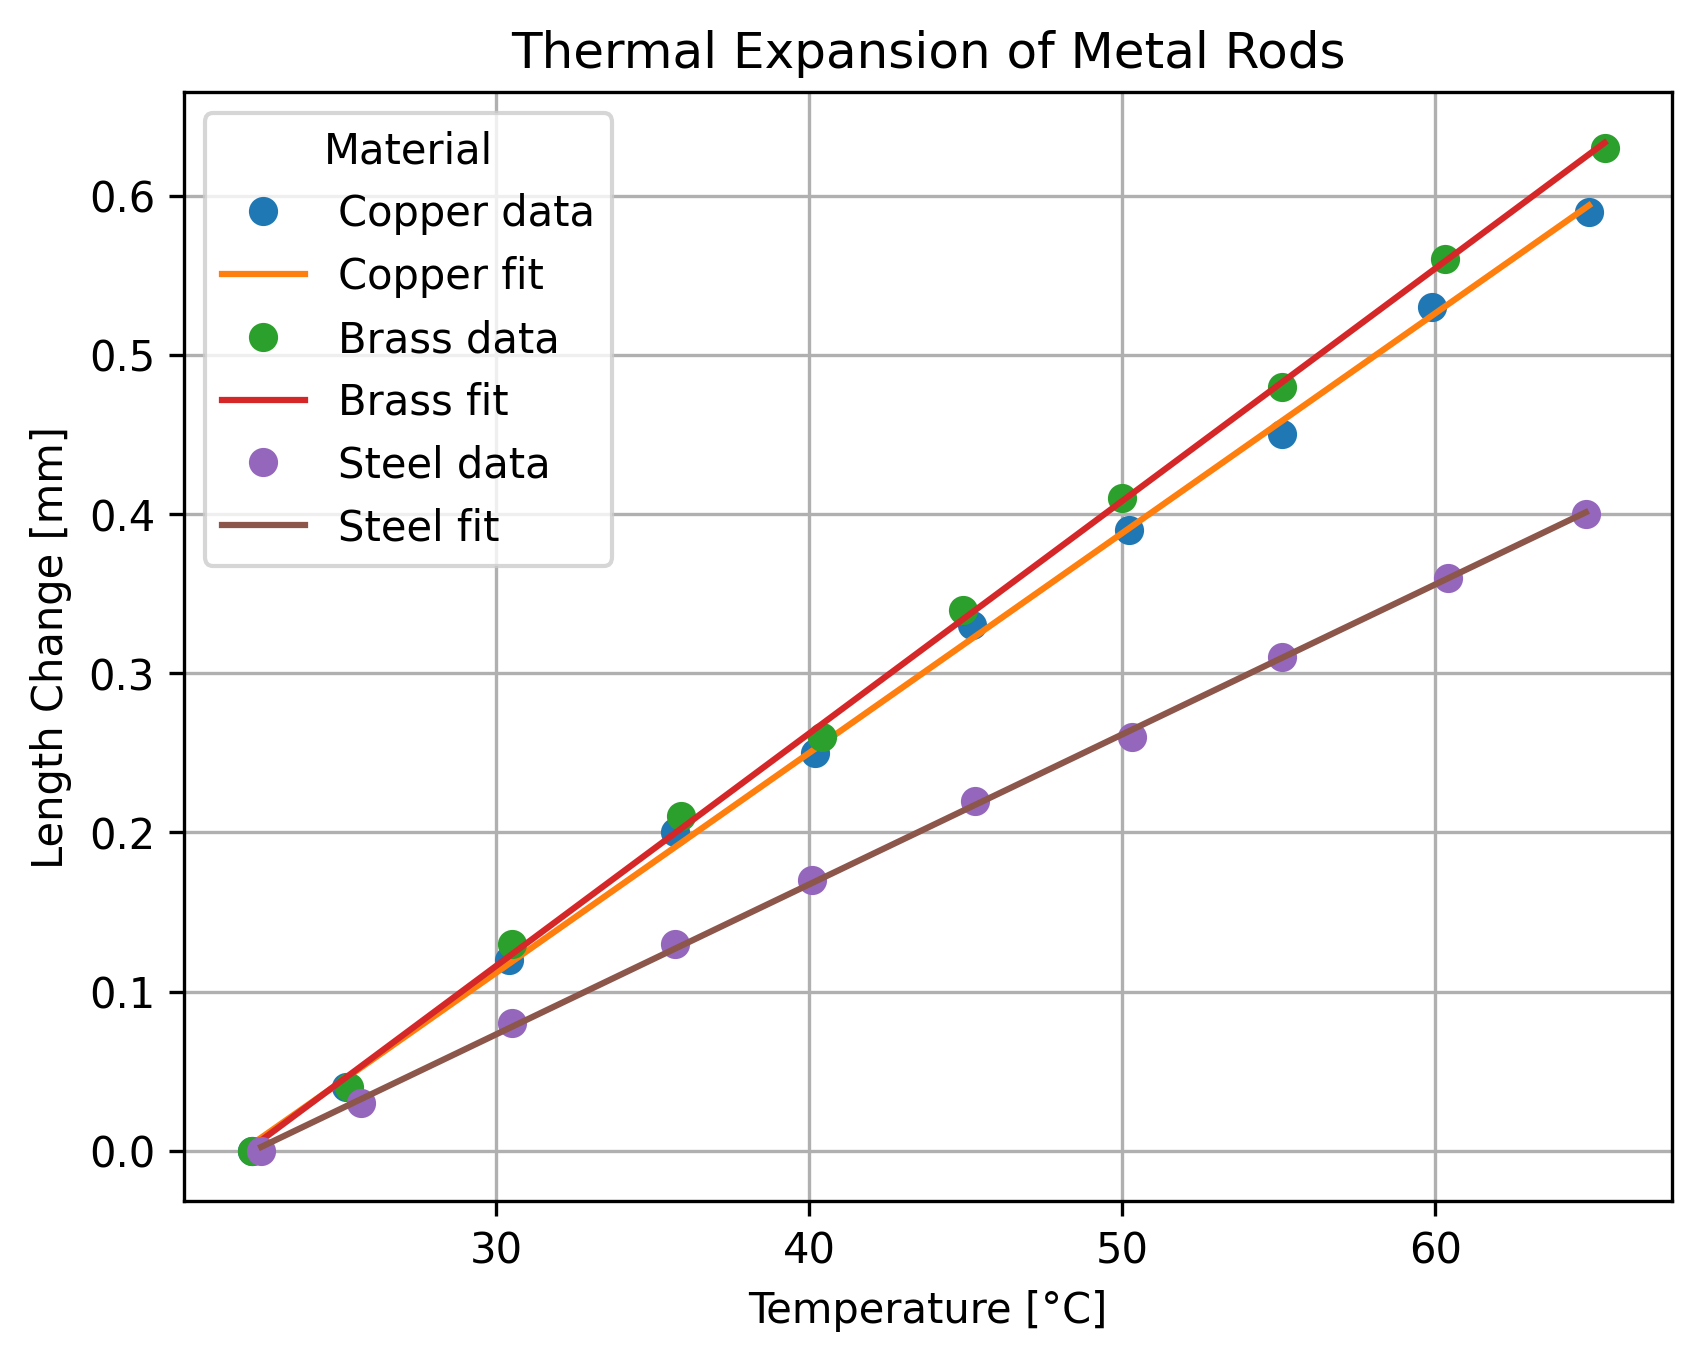
\includegraphics[width=1\textwidth]{expansion_plot.png}
    \caption{Thermal expansion of metal rods.}
    \label{fig:expansion_plot}
\end{figure}

\subsection*{Determined Coefficients}

The coefficients $a$ and the linear expansion coefficient $\alpha$ were calculated using a linear fit of the measured length change $\Delta L$ as a function of temperature $T$ for each metal:

\begin{equation}
    \Delta L = a \, T + b
\end{equation}

Here, $a$ [mm/°C] is the slope of the fitted line, and $b$ is the intercept. The linear expansion coefficient $\alpha$ [1/°C] was then calculated by dividing the slope $a$ by the initial rod length $L_0$:

\begin{equation}
    \alpha = \frac{a}{L_0}
\end{equation}

\begin{table}[H]
\centering
\begin{tabular}{l c c}
\toprule
Metal & $a$ [mm/°C] & $\alpha$ [1/°C] \\
\midrule
Copper & 0.013813 & $1.791 \cdot 10^{-5}$ \\
Brass  & 0.014608 & $1.894 \cdot 10^{-5}$ \\
Steel  & 0.009425 & $1.219 \cdot 10^{-5}$ \\
\bottomrule
\end{tabular}
\caption{Determined linear expansion coefficients.}
\end{table}

\subsection*{Measured Length Changes}

\begin{table}[h]
\centering
\resizebox{\textwidth}{!}{%
\begin{tabular}{c c c}
\csvautotabular[respect all]{measurements.csv}
\end{tabular}
}
\caption{Measured length changes for all three metals.}
\end{table}

\section{Conclusions}

Based on the conducted measurements and data analysis, the following conclusions can be drawn:

\begin{itemize}
    \item All three tested metals exhibit an almost linear relationship between length change and temperature within the examined range.
    \item Brass shows the highest linear expansion, followed by copper, and steel has the lowest.
    \item The determined coefficients $\alpha$ are consistent with typical literature values for these materials.
    \item The linear expansion coefficient allows predicting the rod's length change as a function of temperature, which is important for designing metal structures exposed to temperature fluctuations.
    \item The linear fitting method is appropriate within the range of small temperature changes, where the linear approximation of thermal expansion holds.
\end{itemize}

\end{document}
